%\thispagestyle{myheadings}
\section{Keynote Address: Anton van den Hengel}
\index{van den Hengel, Anton}

\begin{center}
\begin{Large}
  {\bfseries\Large Deep Neural Networks, and what they’re not very good at} \vspace{1em}\par
\end{Large}

%% \begin{center}
%%   \begin{tabular}{m{1in}b{1in}}
%%     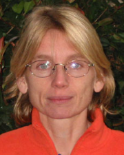
\includegraphics[width=1in]{content/monday/cortes-headshot.png}
%%     & {\bfseries Corinna Cortes} \newline Google Research, NY
%%   \end{tabular}
%% \end{center}

\daydateyear, 9:00--10:00 \vspace{1em}\\
\PlenaryLoc \\
\vspace{1em}\par
%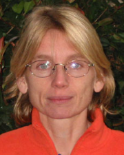
\includegraphics[height=100px]{content/monday/cortes-headshot.png}
\end{center}

\noindent

{\bf Abstract:} Deep Neural Networks have had an incredible impact in a variety of areas within machine learning, including computer vision and natural language processing. Deep Neural Networks use implicit representations that are very high-dimensional, however, and are thus particularly well suited to problems that can be solved by associative recall of previous solutions. They are ill-suited to problems that require human-interpretable representations, explicit manipulation of symbols, or reasoning. The dependency of Deep Neural Networks on large volumes of training data, also means that they are typically only applicable when the problem itself, and the nature of the test data, are predictable long in advance.

The application of Deep Neural Networks to Visual Question Answering has achieved results that would have been thought impossible only a few years ago. It has also thrown a spotlight on the shortcomings of current Deep Nets in solving problems that require explicit reasoning, the use of a knowledge base, or the ability to learn on the fly. In this talk I will illustrate some of the steps being taken to address these problems, and a new learning-to-learn approach that we hope will combine the power of Deep Learning with the significant benefits of explicit-reasoning-based methods.


\vspace{2ex}\centerline{\rule{.5\linewidth}{.5pt}}\vspace{2ex}
\setlength{\parskip}{1ex}\setlength{\parindent}{0ex}

{\bf Biography:} Anton van den Hengel is a Professor in the School of Computer Science at the University of Adelaide, the Director of the Australian Institute for Machine Learning, and a Chief Investigator of the Australian Centre for Robotic Vision. Prof. van den Hengel has been a CI on over \$60m in external research funding from sources including Google, Canon, BHP Billiton and the ARC, and has won a number of awards, including the Pearcey Foundation Entrepreneur Award, the SA Science Excellence Award for Research Collaboration, and the CVPR Best Paper prize in 2010. He has authored over 300 publications, had 8 patents commercialised, formed 2 start-ups, and has recently had a medical technology achieve first-in-class FDA approval. Current research interests include Deep Learning, vison and language problems, interactive image-based modelling, large-scale video surveillance, and learning from large image databases.

\newpage
